\documentclass{article}\usepackage[]{graphicx}\usepackage[]{xcolor}
% maxwidth is the original width if it is less than linewidth
% otherwise use linewidth (to make sure the graphics do not exceed the margin)
\makeatletter
\def\maxwidth{ %
  \ifdim\Gin@nat@width>\linewidth
    \linewidth
  \else
    \Gin@nat@width
  \fi
}
\makeatother

\definecolor{fgcolor}{rgb}{0.345, 0.345, 0.345}
\newcommand{\hlnum}[1]{\textcolor[rgb]{0.686,0.059,0.569}{#1}}%
\newcommand{\hlstr}[1]{\textcolor[rgb]{0.192,0.494,0.8}{#1}}%
\newcommand{\hlcom}[1]{\textcolor[rgb]{0.678,0.584,0.686}{\textit{#1}}}%
\newcommand{\hlopt}[1]{\textcolor[rgb]{0,0,0}{#1}}%
\newcommand{\hlstd}[1]{\textcolor[rgb]{0.345,0.345,0.345}{#1}}%
\newcommand{\hlkwa}[1]{\textcolor[rgb]{0.161,0.373,0.58}{\textbf{#1}}}%
\newcommand{\hlkwb}[1]{\textcolor[rgb]{0.69,0.353,0.396}{#1}}%
\newcommand{\hlkwc}[1]{\textcolor[rgb]{0.333,0.667,0.333}{#1}}%
\newcommand{\hlkwd}[1]{\textcolor[rgb]{0.737,0.353,0.396}{\textbf{#1}}}%
\let\hlipl\hlkwb

\usepackage{framed}
\makeatletter
\newenvironment{kframe}{%
 \def\at@end@of@kframe{}%
 \ifinner\ifhmode%
  \def\at@end@of@kframe{\end{minipage}}%
  \begin{minipage}{\columnwidth}%
 \fi\fi%
 \def\FrameCommand##1{\hskip\@totalleftmargin \hskip-\fboxsep
 \colorbox{shadecolor}{##1}\hskip-\fboxsep
     % There is no \\@totalrightmargin, so:
     \hskip-\linewidth \hskip-\@totalleftmargin \hskip\columnwidth}%
 \MakeFramed {\advance\hsize-\width
   \@totalleftmargin\z@ \linewidth\hsize
   \@setminipage}}%
 {\par\unskip\endMakeFramed%
 \at@end@of@kframe}
\makeatother

\definecolor{shadecolor}{rgb}{.97, .97, .97}
\definecolor{messagecolor}{rgb}{0, 0, 0}
\definecolor{warningcolor}{rgb}{1, 0, 1}
\definecolor{errorcolor}{rgb}{1, 0, 0}
\newenvironment{knitrout}{}{} % an empty environment to be redefined in TeX

\usepackage{alltt}

\usepackage{tikz}
\usetikzlibrary{arrows}
\usetikzlibrary{positioning}
\usetikzlibrary{shapes.geometric}
%\usepackage{wrapfig}     % To wrap text around figures.
\IfFileExists{upquote.sty}{\usepackage{upquote}}{}
\begin{document}  

\title{A Calvin Core 100 Introduction to Sustainability}
\author{Jeremy Van~Antwerp, Matthew Kuperus Heun}

\maketitle

In the long run, sustainability is one of the few things that matter at all.
Sustainability is a challenging problem, in part
because sustainability problems are complex and interconnected,
and because we operate with limited knowledge.
In sustainability, there is tremendous social (and sometimes economic) pressure
to continue to do things ``the way they've always been done.''

Figure~\ref{fig:venn_diagram} shows the three interrelated and overlapping
domains of sustainability:
\textbf{environmental sustainability},
\textbf{economic sustainability}, and
\textbf{social sustainability}.
Sustainability problems are complex and interconnected.
Environmental sustainability problems have social and economic aspects 
(that are generally more difficult to solve).
Likewise, economic and social sustainability problems are not limited to one domain;
typically, they include aspects of the other two domains as well.
Therefore (for example), pollution is an environmental problem, and a social problem, and an economic problem.
Likewise renewable energy. And land use. 
And all the other challenges humanity faces.

\begin{figure}
\centering

  % The next command tells RStudio to do "Compile PDF" on book.Rnw,
% instead of this chapter, thereby eliminating the need to switch back to book.Rnw 
% before making the book.
%!TEX root = ../../book.Rnw

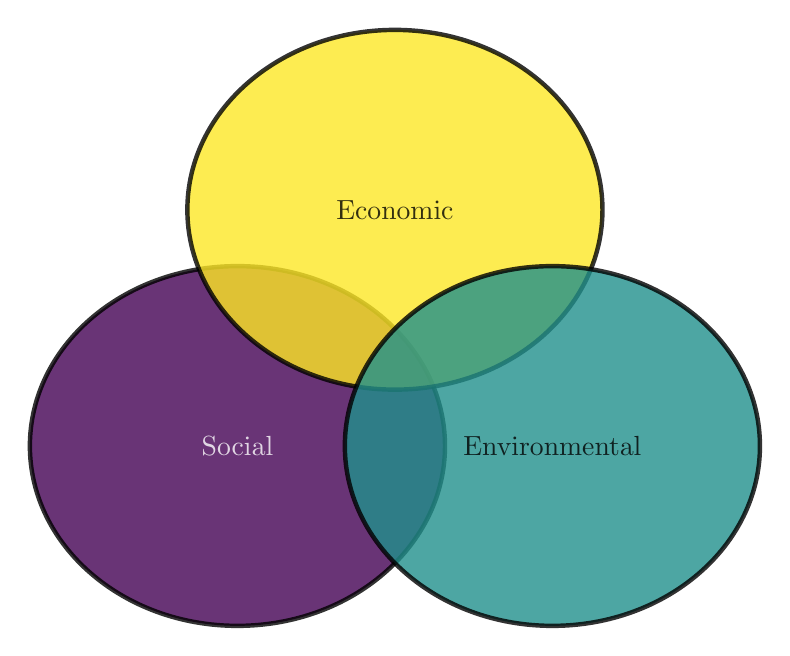
\begin{tikzpicture}
    \definecolor{my_purple}{HTML}{440154}
    \definecolor{my_yellow}{HTML}{FDE725}
    \definecolor{my_green}{HTML}{21908C}
    \tikzstyle{every node}=[ultra thick, ellipse, 
                            minimum width = 150pt,
                            minimum height = 130pt]
    \node[ellipse, draw, fill = my_purple, opacity = 0.8, align = left, text = white] (social) at (-2,0) {Social};
    \node[ellipse, draw, fill = my_yellow, opacity = 0.8, align = center] (economic) at (0,3) {Economic};
    \node[ellipse, draw, fill = my_green, opacity = 0.8, align = right] (environmental) at (2,0) {Environmental};
\end{tikzpicture}


  \caption[Three aspects of sustainability]
          {The three aspects of sustainability.
           Sustainability is often visualized as three overlapping ellipses:
           economic sustainability,
           environmental sustainability, and
           social sustainability.
           The intersecting area represents fully sustainable living.
           Environmental sustainability
           refers to the \textbf{ecosystem} and its supporting services.
           Economic sustainability refers to human systems for creating 
           and accounting for wealth.
           Social sustainability refers to traditions and systems of human society.
           The layering in this figure represents coverage in this book.
           We focus on environmental and
           economic sustainability.
           Social sustainability is vitally important, so it forms the backdrop
           for much of the discussion herein.}
\label{fig:venn_diagram}
\end{figure}


Sustainability is challenging for two additional reasons.
First, it may seem that the changes required to achieve sustainability are so
massively overwhelming that they shouldn't even be addressed.
Second, it may seem like the consequences of not becoming sustainable are so far
in the future that there is neither urgency nor immediate payback.
However, neither of these views is true.
Current news headlines indicate that we are already
experiencing the effects of not being sustainable, in all
sustainability domains---environmentally, economically, and socially.
There are many reasonable and simple things that can be done to improve our
sustainability in the near term.
The deep changes needed for long-term sustainability are urgently needed precisely because
they are long-term investments.
The sooner we begin making those investments, the sooner we'll begin reaping the
rewards and the greater those rewards will be.


\end{document}
